\documentclass[14pt]{beamer}
\usepackage[T2A]{fontenc}
\usepackage[utf8]{inputenc}
%\usepackage[english,russian]{babel}
\usepackage[english]{babel}
\usepackage{booktabs}
\usepackage{tikz}
\usepackage[european,cuteinductors,smartlabels]{circuitikz}
\usetikzlibrary{arrows.meta, shadows}

\usepackage{amssymb,amsfonts,amsmath,mathtext}
\usepackage{amssymb}
\usepackage{cite,enumerate,float,indentfirst}
\usepackage{cancel}
\usepackage{csquotes}
\newcommand{\quotes}[1]{``#1''}
\usetikzlibrary{calc}

\usepackage{mathabx} % rightmoon


\hypersetup{colorlinks,
citecolor=blue,
linkcolor=.,
menucolor=white,
filecolor=pink,   
anchorcolor=yellow
}	    

%\usepackage{pgfplots}
%\usepackage[left=1cm,right=1cm, top=1cm,bottom=1cm,bindingoffset=0cm]{geometry}

% Beamer — верстаем презентации  https://habrahabr.ru/post/145523/ 
\graphicspath{{images/}}



\usetheme{Pittsburgh}
\usecolortheme{whale}

\setbeamercolor{footline}{fg=blue}
\setbeamertemplate{footline}{
\leavevmode%
\hbox{%
\begin{beamercolorbox}[wd=.333333\paperwidth,ht=2.25ex,dp=1ex,center]{}%
Prokshin A.
\end{beamercolorbox}%
\begin{beamercolorbox}[wd=.333333\paperwidth,ht=2.25ex,dp=1ex,center]{}%
Saint-Petersburg, 2019
\end{beamercolorbox}%
\begin{beamercolorbox}[wd=.333333\paperwidth,ht=2.25ex,dp=1ex,right]{}%
p. \insertframenumber{} of \inserttotalframenumber \hspace*{2ex}
\end{beamercolorbox}}%
\vskip0pt%
}

\setbeamertemplate{bibliography item}{[\theenumiv]}

\newcommand{\itemi}{\item[\checkmark]}

	\usefonttheme[onlymath]{serif} % в формулах использовать текст с засечками
\begin{document}
\title{\small{Equipment and automation of solar power plants}}
\author{\small{%
\emph{author:}~Prokshin A}}



\institute{Saint Petersburg Electrotechnical University "LETI"}
\vspace{30pt}%
%Санкт-Петербургский государственный электротехнический университет\\
%«ЛЭТИ» им. В.И. Ульянова (Ленина)

\vspace{60pt}%

%\date{\small{Санкт-Петербург, 2019}}

\AtBeginSection{
	\begin{frame}
		\frametitle{Contents}
		\tableofcontents[currentsection]
	\end{frame}
}

\begin{frame}
\titlepage	
\end{frame}

%\begin{frame}
%        \frametitle{Содержание}
%        \tableofcontents[currentsection] 
%\end{frame}
\begin{frame}
	\frametitle{\small Green Energy (sustainable)}

 living without fossil fuels
	\begin{itemize}
		\item wind
		\item solar
		\begin{itemize}
			\item photovoltaics
			\item thermal
			\item biomass
		\end{itemize}
	\item hydroelectric
	\item wave
	\item tide $\rightmoon$
	\item geothermal
	\end{itemize}
\end{frame}

\begin{frame}
\frametitle{\small PhotoVoltaic} 
PV power engineering has become a meaningful sector of the world economy
%\hspace{-2cm}
	\begin{itemize}
		\item Annual commissioning of PVP capacities has reached 47GW is equivalent \$80bln.(2014) \cite{Morgan}\\
		fact 2019 is: 130GW -- China  , 64.2GW -- US , 0.9GW -- Russia \cite{Morgan,BBC,Chinausfocus,CDU};
\item By 2020 the value of the market will be estimated in terms of \$430-580 bln. 

\end{itemize}
\end{frame}


{
\usebackgroundtemplate{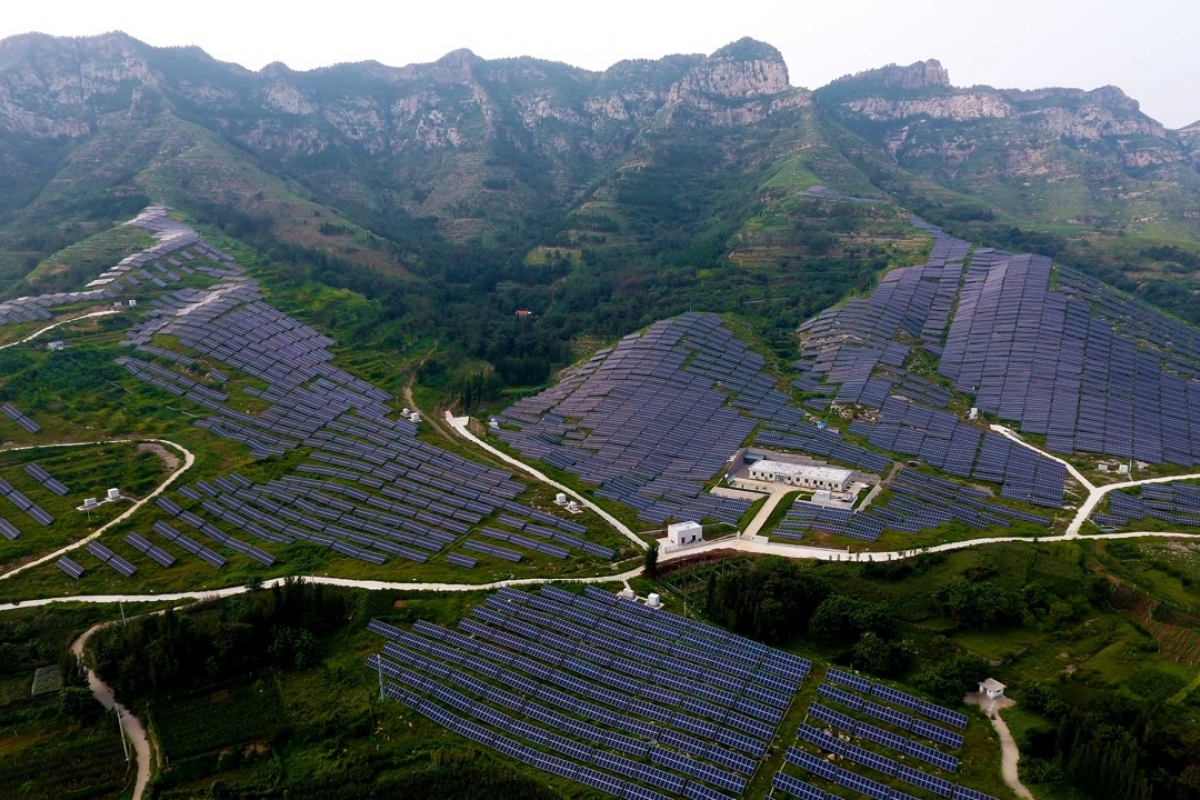
\includegraphics[width=\paperwidth,height=\paperheight]{China_farm.jpg}}	
\begin{frame}
	\frametitle{\small Drivers of the industry growth}
	
	\begin{itemize}
		\item {\color{white}Cost reduction: The improvement of technology;}
		\item {\color{white}Accessibility: The Sun is an inexhaustible;}
		\item {\color{white}Scalability: the size ofa PVP depends on availability of a land plot\cite{ChinaSolorPanelIndustry} and a possibility of system balancing.}
		\item {\color{white}Government support of solar market \cite{SolarEnergyRu}}
	\end{itemize}
\end{frame}
}
\begin{frame}
	\frametitle{\small Grid system balancing}
	%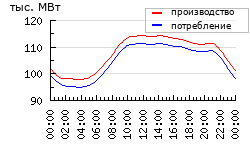
\includegraphics[scale=0.3,width=\paperwidth/4,height=\paperheight/4]{2019-08-10_1_2_1019.png}
	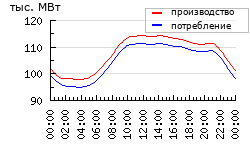
\includegraphics[scale=0.6]{2019-08-10_1_2_1019.png}
	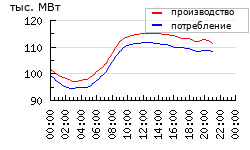
\includegraphics[scale=0.6]{2019-08-10_1_4_1019.png}
	Plan and facts of generation and consuming (daytime, temperature, wind).

        Balance of active and reactive power, overall system stability. Some time you have to switch off generation. 
\end{frame}	

\begin{frame}
	\frametitle{\small Government support of solar market}
	plans:
	\begin{itemize}
		\item Green Energy program 2015-2025  -- 5 GW (70\% -- wind, the rest solar and small hydro- )
		\item Green Energy program	2025-2035  5.5 GW
        	\item presumable after 2035 wind/solar generations  will not need explicit Gov. support 
	\end{itemize}
	implemetnation(financial tools):	

companies that acquired rights to place Power Purchase Agreements (PPA) contracts and construct generating capacity in 10 regions of Russia.

concurent aquiring of power.

\end{frame}


\begin{frame}
In comparision:

	\href{https://www.youtube.com/watch?v=855Am6ovK7s&feature=youtu.be&t=920}{1st Debates, The Clean Energy Superpower}

	\href{https://youtu.be/FRlI2SQ0Ueg?t=4980}{2nd Debates, One question about energy policy}


In total, under the Trump Administration, the US solar sector has lost almost 20,000 jobs. 
Meanwhile, according to the IRENE Renewable Energy and Jobs 2018 Report, 
China’s solar industry has continued to expand by 13\% over the previous year. 
\end{frame}	

\begin{frame}
China, 2017 -- 53 GW capacity installed

China, 2018 -- 35 GW capacity installed

	Russia, (mainly Hevel)

Samara 75 mW (this summer),

%https://rg.ru/2019/05/22/reg-pfo/pod-samaroj-zapustili-krupnejshuiu-v-strane-solnechnuiu-elektrostanciiu.html
Crimea, 5 SES, 297mW
	%https://ru.wikipedia.org/wiki/%D0%90%D0%BB%D1%8C%D1%82%D0%B5%D1%80%D0%BD%D0%B0%D1%82%D0%B8%D0%B2%D0%BD%D0%B0%D1%8F_%D1%8D%D0%BD%D0%B5%D1%80%D0%B3%D0%B5%D1%82%D0%B8%D0%BA%D0%B0_%D0%9A%D1%80%D1%8B%D0%BC%D0%B0
	Altai, 1 april, Ininskaya-10mW, Mayminskaya-5mW, (now 8 SES capacity 65Mw, at 2020 - 125mW)
	%https://neftegaz.ru/news/Alternative-energy/347216-v-respublike-altay-vvedeny-v-ekspluatatsiyu-2-solnechnye-elektrostantsii/
	%https://iz.ru/866177/2019-04-10/novye-solnechnye-elektrostantcii-poiaviatsia-v-respublike-altai-k-2020-godu
% СЭС: Кош-Агачская СЭС, Кош-Агачская СЭС-2, Усть-Канская СЭС, Онгудайская СЭС, Майминская СЭС (1я и 2я очереди), Майминская СЭС-3 и Ининская СЭС.
%Это позволило избежать 25 тыс. т выбросов углекислого газа в атмосферу и сэкономить 13,8 млн м3 природного газа. 
	Tuva, Mongun-Taiginsky district 600kW % Монгун-Тайгинском район, 600kW, (up to 1.6MW)
\end{frame}

\begin{thebibliography}{7}
\begin{frame}
\frametitle{\small References}
	\tiny{ 
\bibitem{Morgan} Byrd, S. et al. 2014, “Solar Power \& Energy Storage”, Morgan Stanley 
	\bibitem{BBC} How China's giant solar farms are transforming world energy \url{www.bbc.com/future/story/20180822-why-china-is-transforming-the-worlds-solar-energy}
	\bibitem{Chinausfocus}	U.S. Solar Industry Shaken by Trump’s Trade War \url{www.chinausfocus.com/finance-economy/us-solar-industry-shaken-by-trumps-trade-war}
	\bibitem{CDU} System Operator of the United Power System, Joint-stock Company  \url{www.so-ups.ru/index.php?id=ees}	
	\bibitem{SolarEnergyRu}	\url{http://www.sol-en.ru/en/energy/wholesale_market}
	\bibitem{ChinaSolorPanelIndustry} \url{www.scmp.com/business/companies/article/2137539/chinas-solar-panel-industry-faces-year-reckoning-amid-global}
	\bibitem{NY} \url{https://www.nyserda.ny.gov/About/Tracking-Progress/Clean-Energy-Powers-New-York}
	\bibitem{Car} Electric vehicle charging increased  \url{https://www.nyserda.ny.gov/About/Tracking-Progress/Clean-Energy-Powers-New-York}
	\bibitem{Gargantuan} \url{https://www.climatecentral.org/news/china-solar-farm-satellite-21182}
	\bibitem{EE} \url{https://electricenergyonline.com}
		}
\end{frame}
\begin{frame}
	\tiny{
%        \bibitem{Sokolovsky}Соколовский Г.Г. Электроприводы переменного тока с частотным регулированием: Учебник для студ. высш.учеб.заведений.  -- М. «Академия», 2007 - 272 с.
%	\bibitem{Zagruzchik}Программа-загрузчик \url{github.com/rogerclarkmelbourne/Arduino\_STM32}
%	\bibitem{MexBios}Мехбиос \url{http://www.mechatronica-pro.com}
%	\bibitem{ControlSUITE} \url{https://www.ti.com/tool/CONTROLSUITE}
		%описание на русском https://habr.com/post/403007/\\
%на английском %http://www.rogerclark.net/stm32f103-and-maple-maple-mini-with-arduino-1-5-x-ide/
%
%       Сама  программа загрузчик -- \\
%{\small https://github.com/rogerclarkmelbourne/Arduino\_STM32}


}
\end{frame}
\end{thebibliography}
\end{document}

